\section{Implementazione}
\todo{Parlare del domain model, delle annotazioni, dei repository, dei service forse è più adatto qui parlare approfonditamente del databse ed in progettazione fare un introduzione}
\todo[color=blue]{Qui parla di come hai implementato il transaction manager, E Gui approfondita}
In questa sezione verrà descritta l'implementazione dell'applicazione analizzandone tutti
i componenti.
\subsection{Domain Model}
\begin{figure}
    \centering
    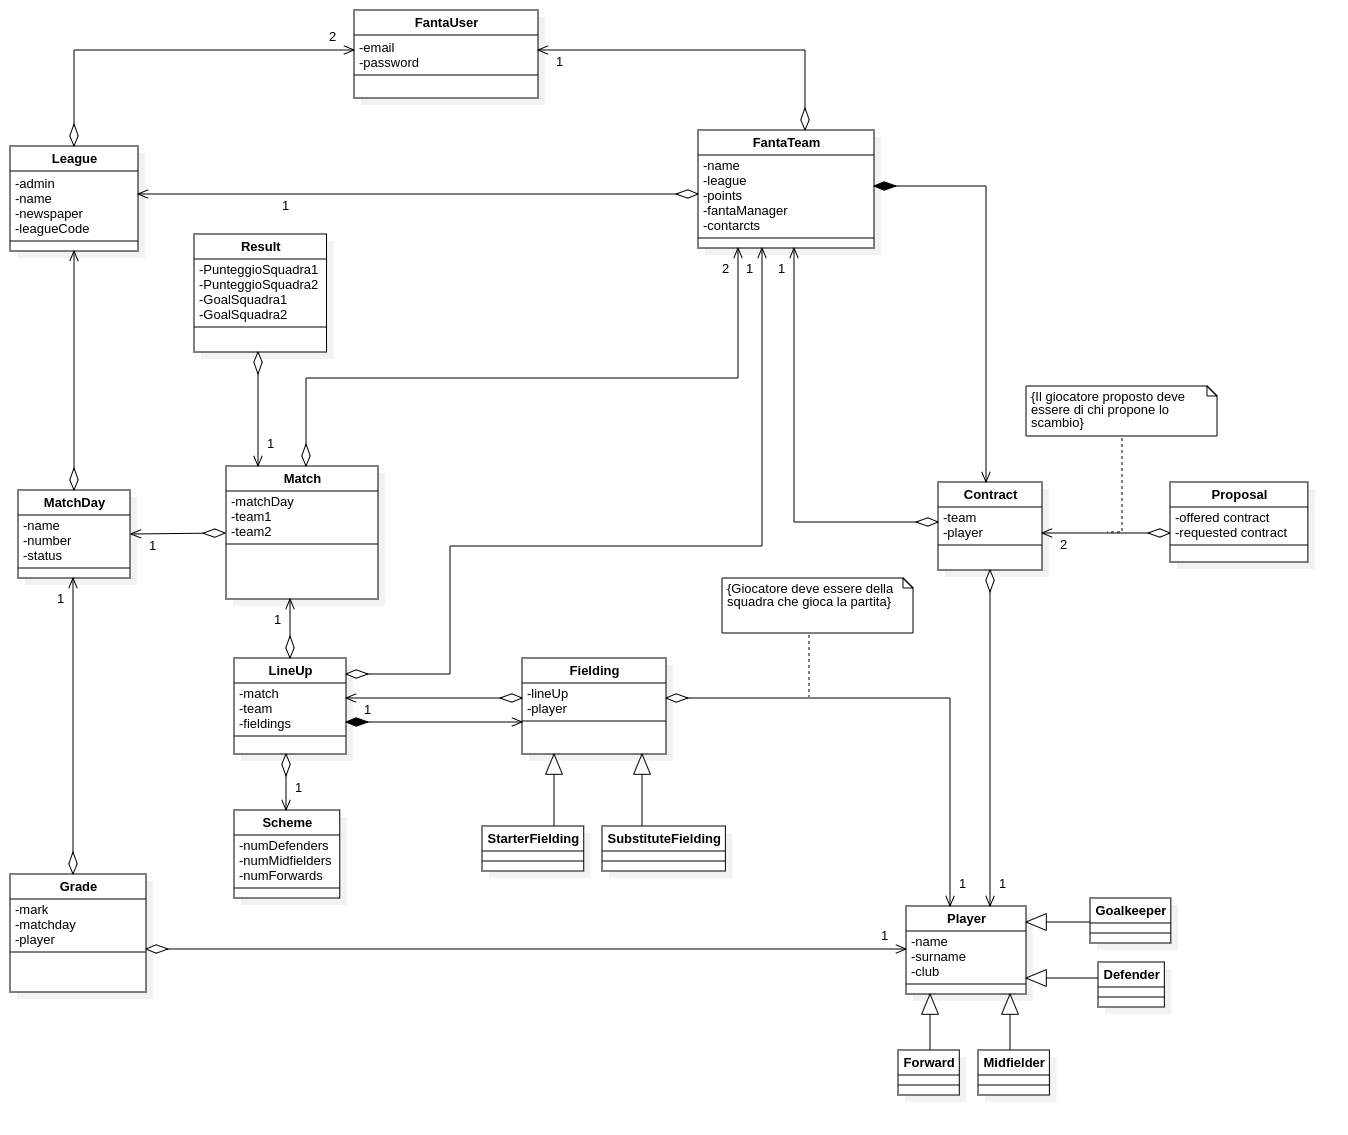
\includegraphics[width=\textwidth]{Resources/graficiUML/ClassDiagram.png}        
    \caption{Domain class diagram.}
    \label{fig:domain_class_diagram2}
\end{figure}
Il domainn model rappresnta le entità di dominio del sistema e le loro relazioni.
Tutte le classi presenti sono state annotate con \textbf{Jpa}.
La classe \textbf{League} rappresenta la lega. Essa ha un nome, un codice ed un riferimento
a due user l'admin e il journalist. La classe \textbf{fantaUser} rappresenta l'utente che può
svolgere varie azioni in base al ruolo che ricopre nella lega. La classe \textbf{FantaTeam}
rappresenta il team di un utente all'interno di una lega. È interessante riportare
che la classe \textbf{FantaTeam} ha una relazione bidirezionale con la classe \textbf{Contract},
ciò è sato implementato con la relazione \textbf{Jpa MappedBy}, nella sezione su \textbf{Jpa}
sono stati approfonditi i motivi di questa scelta.Inoltre è presente la classe \textbf{FantateamViewer}
che non è nient'altro che un visitor per estrarre il calciatori di un team in base al ruolo. La classe \textbf{Contract} rappresenta l'assegnazione di un
calciatore ad un determinato team. La classe \textbf{Proposal} rappresenta la proposta di scambio
di due calciatori appartenenti a due team della stessa lega. La classe \textbf{Player} rappresenta il calciatore. Il
campo \textit{club} del calciatore rappresenta la squadra reale ed è realizzata con un enum.
Per distinguere tra i vari ruoli di un calciatore abbiamo deciso di creare delle sottoclassi per ognuno di essi,
in questo modo si possono aggiungere ulteriori ruoli per rendere più realistico il gioco.
Per rappresentare le giornate da giocare di una specifica lega è presente la classe \textbf{Matchday}. Ogni giornata è numerata
ed ha uno status rappresentato tramite un enum, in questo modo è possibile stabilire lo stato di avanzamento del gioco
per quella determinata lega. Ad ogni match day sono associati i voti dei calciatori
assegnati dal giornalista, la classe che rappresenta ciò è \textbf{Grade}.
In ogni giornata sono presenti più match ognuno dei quali è rappresentato 
dalla classe \textbf{Match}. Ogni match ha il riferimento ai due team coinvolti
ed una volta concluso ha un riferimento alla classe \textbf{Result}, ovvero il suo risultato.
La classe \textbf{LineUp} rappresenta la formazione schierata da un team per un match.
La classe \textbf{Scheme}, che rappresenta il modulo, è utilizzata per fare type mapping di \textbf{LineUp}. Anche per \textbf{LineUp} è presente una relazione mapppata
con \textbf{Jpa MappedBy} ed è quella con \textbf{Fielding}, che rappresenta lo schiaremento di un giocatore.
Infine è presente una classe \textbf{LineUpViewer} che implementa un'api sequenziabilizzabile e sicura
per instanziare una \textbf{LineUp}.

\subsection{Services}
Nel pacchetto \textit{Business} sono presenti i services, uno per ogni tipo di attore ed uno per il login.
I services utilizzano il \textbf{TransactionManager} per gestire le transazioni con il database.
In particolare vengono utilizzati i due metodi \textit{inTransaction} e \textit{fromTransaction}, il primo esegue la funzione
 passata all'interno di una transazione e non restituisce nulla mentre il secondo restituisce
 il valore della funzione passata. Inoltre attraverso il \textbf{TransactionContext} i services
 sono in grado di utilizzare i repository per effettuare le loro operazioni.
 I services presenti sono:
 \begin{itemize}
    \item \textbf{LoginService}: si occupa di effettuare le operazioni di login e registrazione.
    \item \textbf{UserService}: si occupa di gestire le operazioni di un utente base all'interno di una lega in cui partecipa.
    \item \textbf{AdminUserService}: si occupa gi gestire le operazioni esclusive di un admin all'interno di una lega.
    \item \textbf{NewsPaperService}: si occupa di gestire le operazioni di un giornalista all'interno di una lega.
 \end{itemize}

\begin{figure}
    \centering
    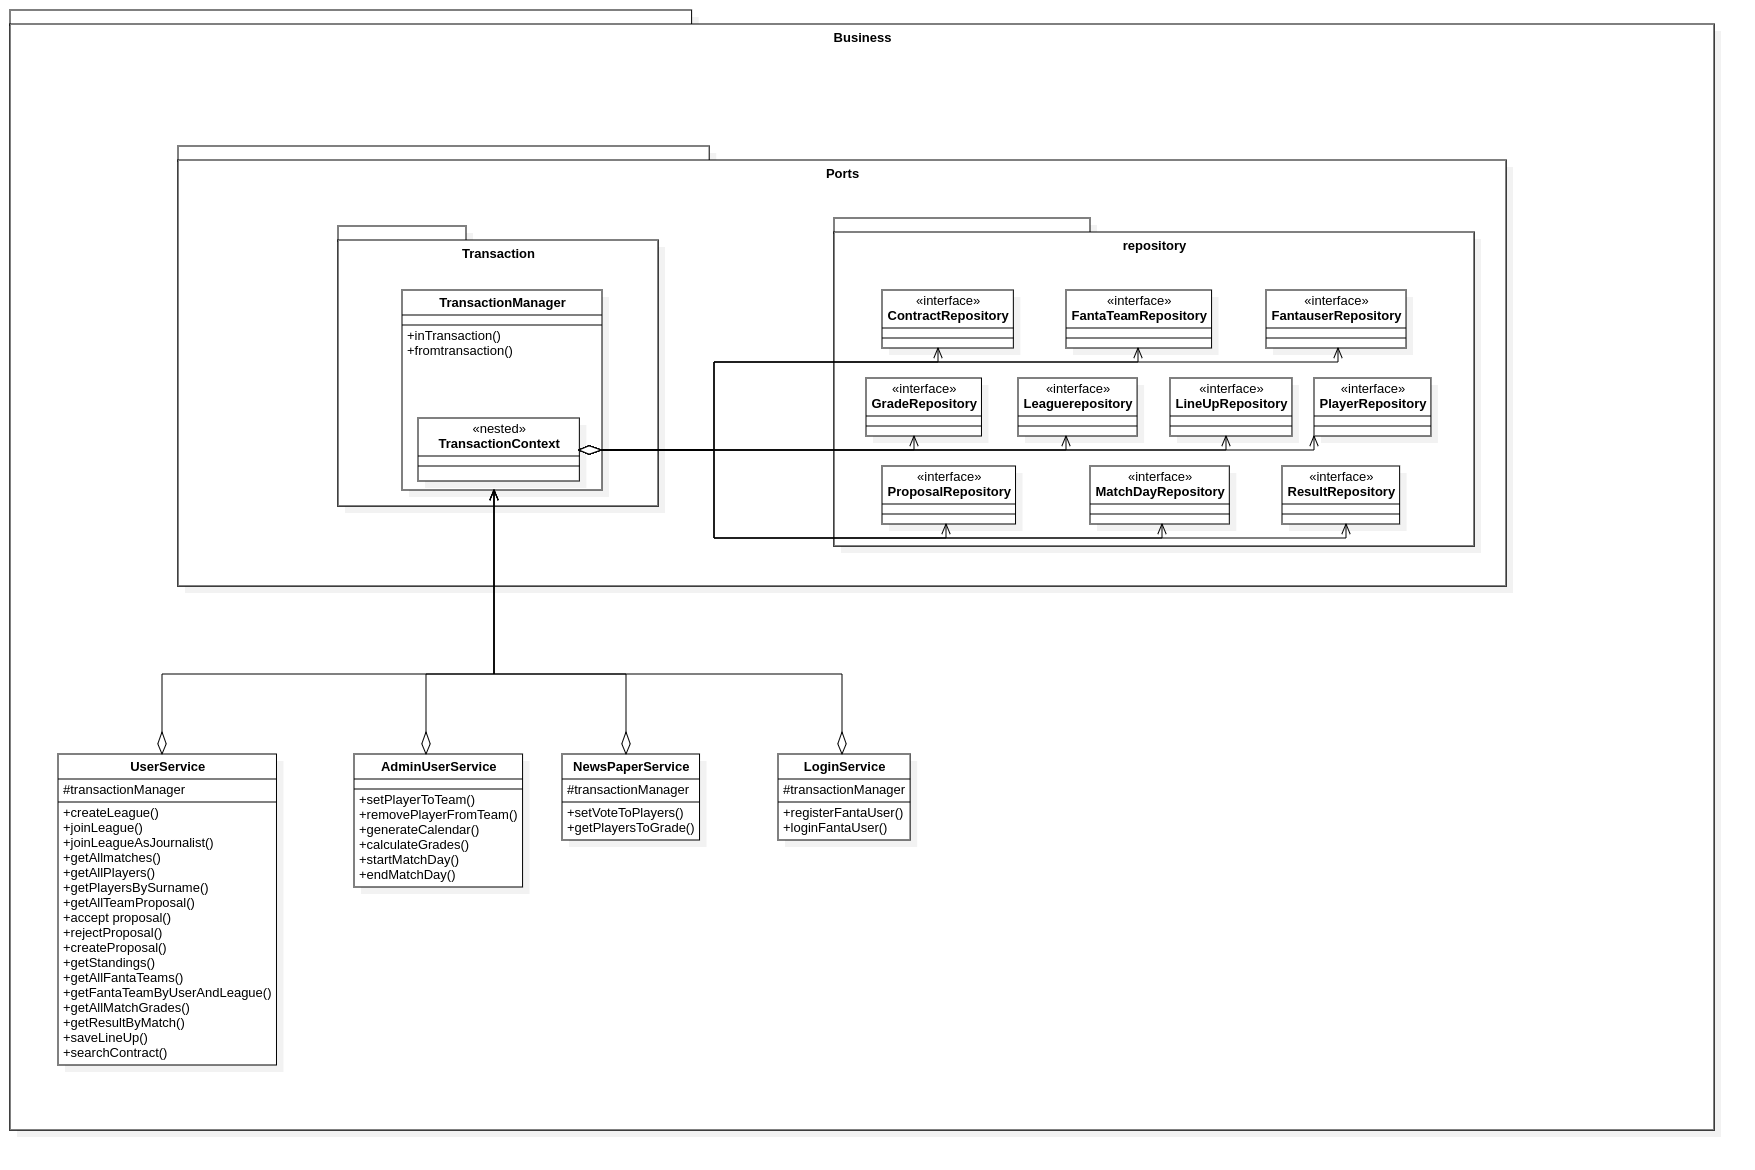
\includegraphics[width=\textwidth]{Resources/graficiUML/BusinessClassDiagram.png}        
    \caption{Business class diagram.}
    \label{fig:business_class_diagram2}
\end{figure}

Di seguito l'implementazione di \textit{inTransaction} e \textit{fromTransaction}:
\begin{lstlisting}[language=Java]
@Override
	public <T> T fromTransaction(Function<TransactionContext, T> code) {

		EntityManager em = emFactory.createEntityManager();
		EntityTransaction transaction = em.getTransaction();
		try {
			transaction.begin();
			T result = code.apply(new TransactionContext(
										new JpaLeagueRepository(em), 
										new JpaMatchRepository(em),
										new JpaPlayerRepository(em), 
										new JpaFantaTeamRepository(em), 
										new JpaGradeRepository(em),
										new JpaProposalRepository(em), 
										new JpaContractRepository(em), 
										new JpaResultsRepository(em),
										new JpaFieldingRepository(em), 
										new JpaLineUpRepository(em), 
										new JpaMatchDayRepository(em),
										new JpaNewsPaperRepository(em), 
										new JpaFantaUserRepository(em)));
			transaction.commit();
			return result;
		} catch (Exception e) {
			if (transaction.isActive()) {
				transaction.rollback();
			}
			throw e;
		} finally {
			em.close();
		}
	}

	@Override
	public void inTransaction(Consumer<TransactionContext> code) {
		fromTransaction((context) -> {
			code.accept(context);
			return true;
		});
	}
}
\end{lstlisting}
\newpage

\subsection{Repositories}
I repository concreti estendono tutti il \textbf{BaseJpaRepository} ed implementano la relativa interfaccia.
Le query sono state implementate con le \textit{CriteriaQuery}, ciò ha permesso insieme
all'utilizzo del metamodello di avere un controllo a compile time sulle entità utilizzate nella query.

\begin{figure}
    \centering
    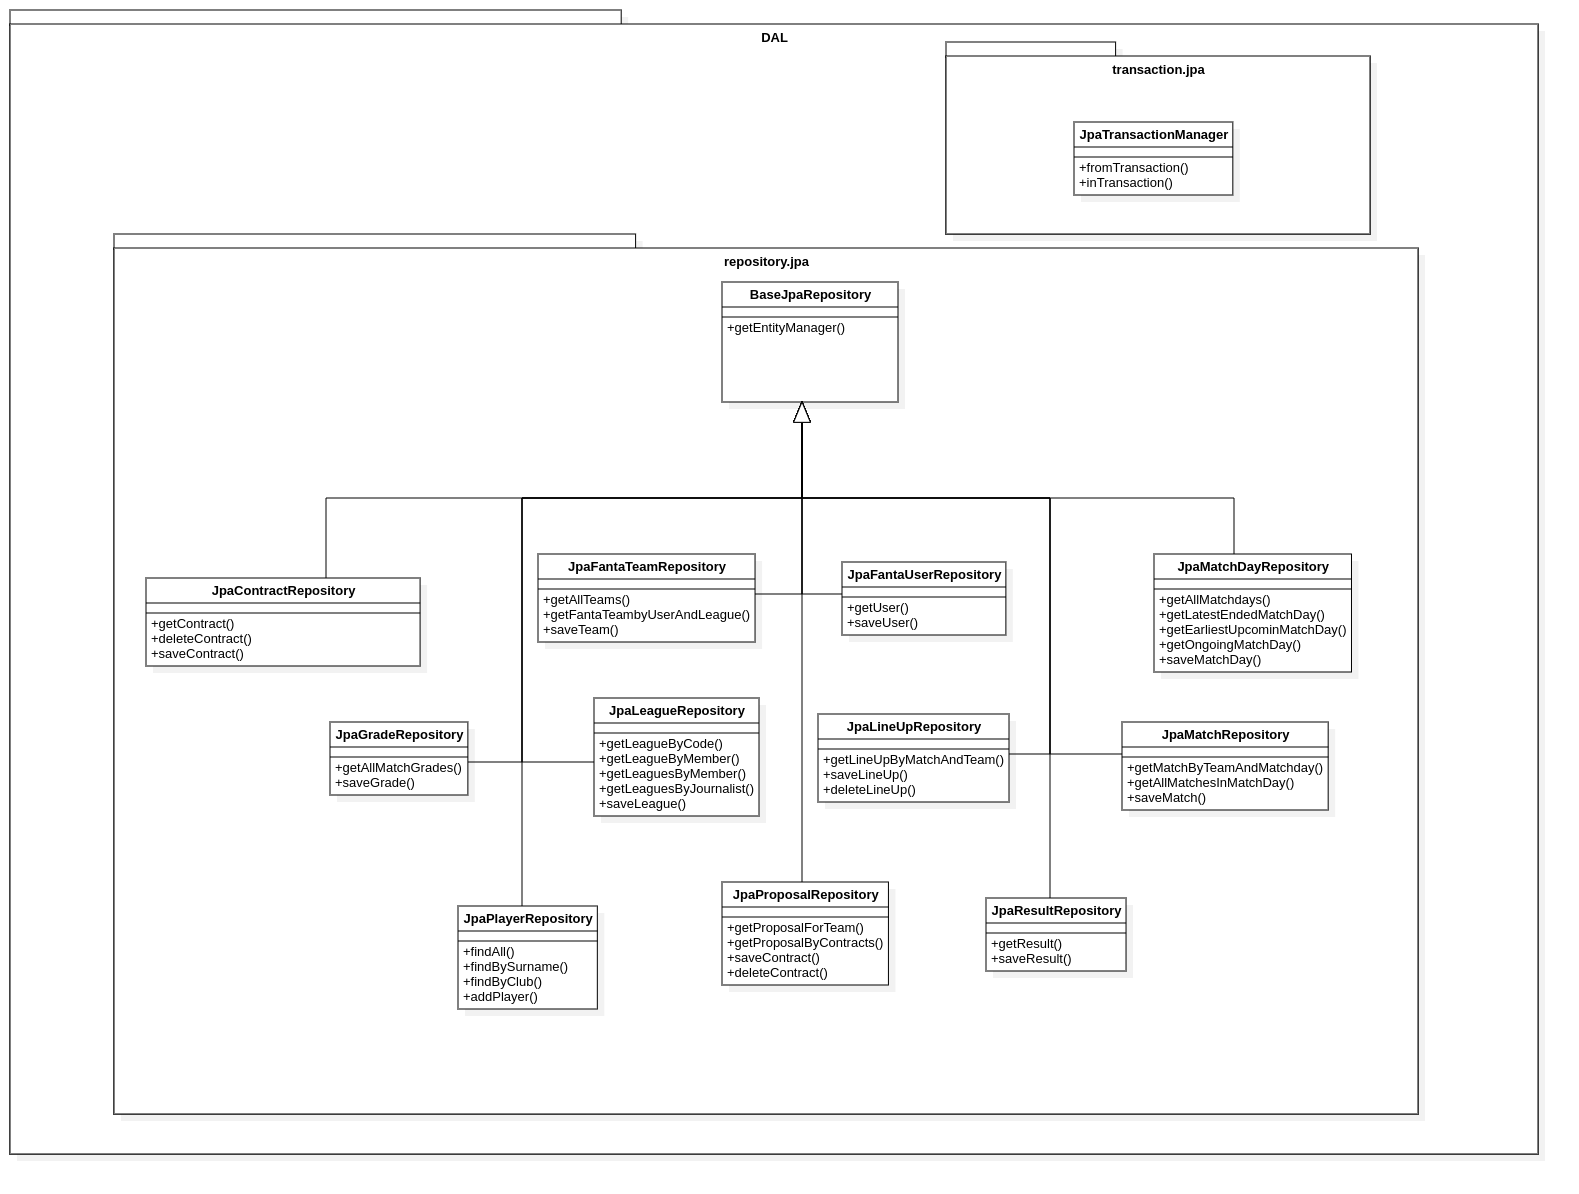
\includegraphics[width=\textwidth]{Resources/graficiUML/DALClassDiagram.png}        
    \caption{Dal class diagram.}
    \label{fig:Dal_class_diagram2}
\end{figure}

Esempio di query effettuata tramite le \textit{CriteriaQuery}:
\begin{lstlisting}[language=Java]
@Override
	public Optional<FantaUser> getUser(String email, String password) {
    	EntityManager em = getEntityManager();
        CriteriaBuilder cb = em.getCriteriaBuilder();
        CriteriaQuery<FantaUser> query = cb.createQuery(FantaUser.class);
        Root<FantaUser> root = query.from(FantaUser.class);

        query.select(root).where(
                cb.equal(root.get(FantaUser_.email), email),
                cb.equal(root.get(FantaUser_.password), password)
        );

        return em.createQuery(query).getResultList().stream().findFirst();
	}
}
\end{lstlisting}